%% beamer packages
% other themes: AnnArbor, Antibes, Bergen, Berkeley, Berlin, Boadilla, boxes, 
% CambridgeUS, Darmstadt, Dresden, Frankfurt, Goettingen, Hannover, Ilmenau,
%JuanLesPins, Luebeck, Madrid, Malmoe, Marburg, Montpellier, PaloAlto,
%Pittsburgh, Rochester, Singapore, Szeged, Warsaw
% other colors: albatross, beaver, crane, default, dolphin, dove, fly, lily, 
%orchid, rose, seagull, seahorse, sidebartab, structure, whale, wolverine,
%beetle

%\documentclass[xcolor=dvipsnames]{beamer}
\documentclass[table,dvipsnames]{beamer}
\usepackage{beamerthemesplit}
\usepackage{bm,amsmath,marvosym}
\usepackage{listings,color}%xcolor
\usepackage[ngerman]{babel}
\usepackage{natbib}
\usepackage[utf8]{inputenc}
\definecolor{shadecolor}{rgb}{.9, .9, .9}
\definecolor{darkblue}{rgb}{0.0,0.0,0.5}
\definecolor{myorange}{cmyk}{0,0.7,1,0}
\definecolor{mypurple}{cmyk}{0.3, 0.9, 0.0, 0.2}

% make a checkmark
\usepackage{tikz}
\def\checkmark{\tikz\fill[scale=0.4](0,.35) -- (.25,0) -- (1,.7) -- (.25,.15) -- cycle;} 

% dot product
\usetikzlibrary{arrows,positioning}
\tikzset{
    %Define standard arrow tip
    >=stealth',
    % Define arrow style
    pil/.style={->,thick}
}

% math stuff
\newcommand{\argmin}{\operatornamewithlimits{argmin}}

\lstnewenvironment{code}{
    \lstset{backgroundcolor=\color{shadecolor},
        showstringspaces=false,
        language=python,
        frame=single,
        framerule=0pt,
        keepspaces=true,
        breaklines=true,
        basicstyle=\ttfamily,
        keywordstyle=\bfseries,
        basicstyle=\ttfamily\scriptsize,
        keywordstyle=\color{blue}\ttfamily,
        stringstyle=\color{red}\ttfamily,
        commentstyle=\color{green}\ttfamily,
        columns=fullflexible
    }
}{}

\lstnewenvironment{codeout}{
    \lstset{backgroundcolor=\color{shadecolor},
        frame=single,
        framerule=0pt,
        breaklines=true,
        basicstyle=\ttfamily\scriptsize,
        columns=fullflexible
    }
}{}

\hypersetup{colorlinks = true, linkcolor=darkblue, citecolor=darkblue,urlcolor=darkblue}
\hypersetup{pdfauthor={A. Richards}, pdftitle={Intro to probabilistic programming}}

\newcommand{\rd}{\textcolor{red}}
\newcommand{\grn}{\textcolor{green}}
\newcommand{\keywd}{\textcolor{myorange}}
\newcommand{\highlt}{\textcolor{NavyBlue}}
\newcommand{\norm}[1]{\left\lVert#1\right\rVert}
\def\ci{\perp\!\!\!\perp}
% set beamer theme and color
\usetheme{Frankfurt}
%\usetheme{Berkeley}
\usecolortheme{orchid}
%\usecolortheme{seagull}

%% modify the font
%\usepackage{fontspec}
%setting a font
%\setsansfont{TeX Gyre Adventor}
%\usepackage{newcent}

%% fix the section title for literature
\renewcommand{\bibsection}{\subsubsection*{\bibname } }

\title[Project teams]{Introduction to probabilistic programming \\ (Introducing our new friend Edward)}
\author[A. Richards]{Adam Richards \\ \ \\ 
\includegraphics[scale=0.05]{galvanize-logo.png}}
\institute{}
\date[]{01.04.2018}

%%%%%%%%%%%%%%%%%%%%%%%%%%%%%%%%%%%%%%%%%%%%%%%%%%%%%%%%%%%%%%%%%%%%%%%%%%%%%%%
\begin{document}
\frame{\titlepage}
%%%%%%%%%%%%%%%%%%%%%%%%%%%%%%%%%%%%%%%%%%%%%%%%%%%%%%%%%%%%%%%%%%%%%%%%%%%%%%%
\frame{
\footnotesize
\tableofcontents
\normalsize
}

%%%%%%%%%%%%%%%%%%%%%%%%%%%%%%%%%%%%%%%%%%%%%%%%%%%%%%%%%%%%%%%%%%%%%%%%%%%%%%%
\section{Probabilistic Programming}
\subsection{}

%%%%%%%%%%%%%%%%%%%%%%%%%%%%%%%%%%%%%%%%%%%%%%%%%%%%%%%%%%%%%%%%%%%%%%%%%%%%%%%
\frame{   
\frametitle{What are we going to cover?}
\begin{block}{}
 \begin{itemize}
  \item Probabilistic programming intro 
  \item Box's Loop (Model $\rightarrow$ infer $\rightarrow$ criticize)
  \item Bayesian inference and some related tools
  \item Examples in both PyMC3 and Edward (model)
  \item Discuss the tools used for inference and criticism 
  \item Switchpoint and multilevel modeling examples
  \end{itemize}
\end{block}
}

%%%%%%%%%%%%%%%%%%%%%%%%%%%%%%%%%%%%%%%%%%%%%%%%%%%%%%%%%%%%%%%%%%%%%%%%%%%%%%%
\frame{   
\frametitle{Probabilistic programming}
\footnotesize
\begin{block}{A probabilistic programming language makes it easy to:}
 \begin{enumerate}
  \item Write out complex probability models
  \item And subsequently solve these models automatically.
 \end{enumerate}
 \end{block}

\begin{block}{Generally this is accomplished by:}
 \begin{enumerate}
  \item Random variables are handled as a \href{https://en.wikipedia.org/wiki/Language\_primitive}{primitive}
  \item Inference is handled behind the scenes
  \item Memory and processor management is abstracted away
 \end{enumerate}
 \end{block} 
}

%%%%%%%%%%%%%%%%%%%%%%%%%%%%%%%%%%%%%%%%%%%%%%%%%%%%%%%%%%%%%%%%%%%%%%%%%%%%%%%
\frame{ 
\frametitle{The pros and the cons}
\footnotesize
\textbf{Why you might want to use probabilistic programming}
\begin{enumerate}
 \item \keywd{Customization} - We can create models that have built-in hypothesis tests
 \item \keywd{Propagation of uncertainty} - There is a degree of belief associated prediction and estimation
 \item \keywd{Intuition} - The models are essentially 'white-box' which provides insight into our data
\end{enumerate}
\textbf{Why you might \highlt{NOT} want use out probabilistic programming}
\begin{enumerate}
 \item \keywd{Deep dive} - Many of the online examples will assume a fairly deep understanding of statistics
 \item \keywd{Overhead} - Computational overhead might make it difficult to be production ready
 \item \keywd{Sometimes simple is enough} - The ability to customize models in almost a plug-n-play manner has to come with some cost. 
\end{enumerate}
}


%%%%%%%%%%%%%%%%%%%%%%%%%%%%%%%%%%%%%%%%%%%%%%%%%%%%%%%%%%%%%%%%%%%%%%%%%%%%%%%
\frame{
\frametitle{Doing data science}
\footnotesize
The taxonomy of what a data scientist does
\begin{columns}
 
\begin{column}{6cm}
\begin{enumerate}
 \item Obtaining data
 \item Scrubbing data
 \item Exploring data
 \item Modeling data
 \item iNterpreting data
\end{enumerate}
\vspace{1cm}
OSEMN is pronounced as \keywd{Awesome}.
\end{column}
\begin{column}{5cm}
\begin{center}
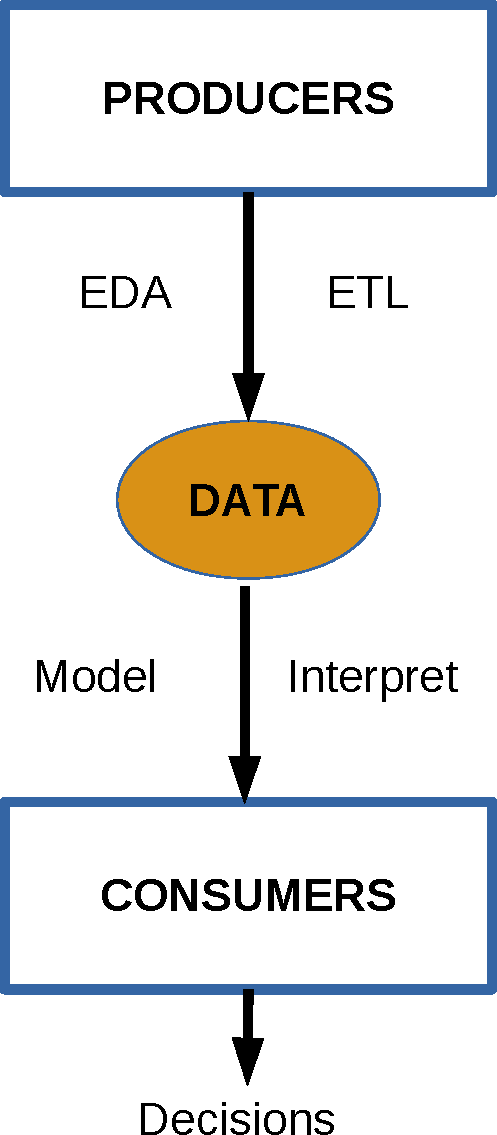
\includegraphics[scale=0.3]{data-decisions.pdf}
\end{center}
\end{column}
\end{columns}


\tiny
\begin{flushleft}
See Hilary Mason and Chris Wiggins blog post \\
\href{http://www.dataists.com/2010/09/a-taxonomy-of-data-science}{http://www.dataists.com/2010/09/a-taxonomy-of-data-science}
\end{flushleft}
}

%%%%%%%%%%%%%%%%%%%%%%%%%%%%%%%%%%%%%%%%%%%%%%%%%%%%%%%%%%%%%%%%%%%%%%%%%%%%%%%
\frame{ 
\frametitle{probabilistic programming and data science}
\footnotesize
\begin{columns}
\begin{column}{5.5cm}
\begin{center}
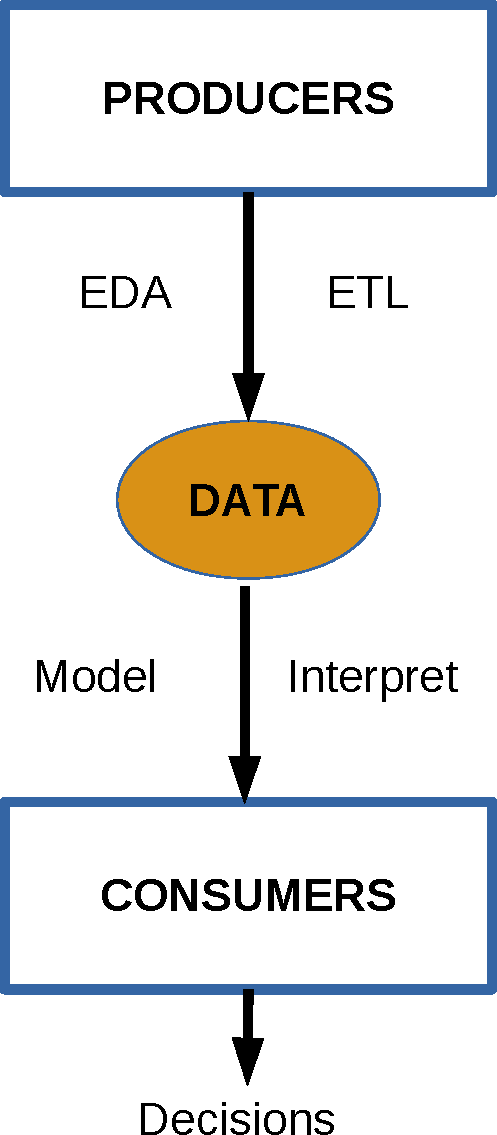
\includegraphics[scale=0.3]{data-decisions.pdf}
\end{center}
\end{column}

\begin{column}{5.5cm}
\begin{center}
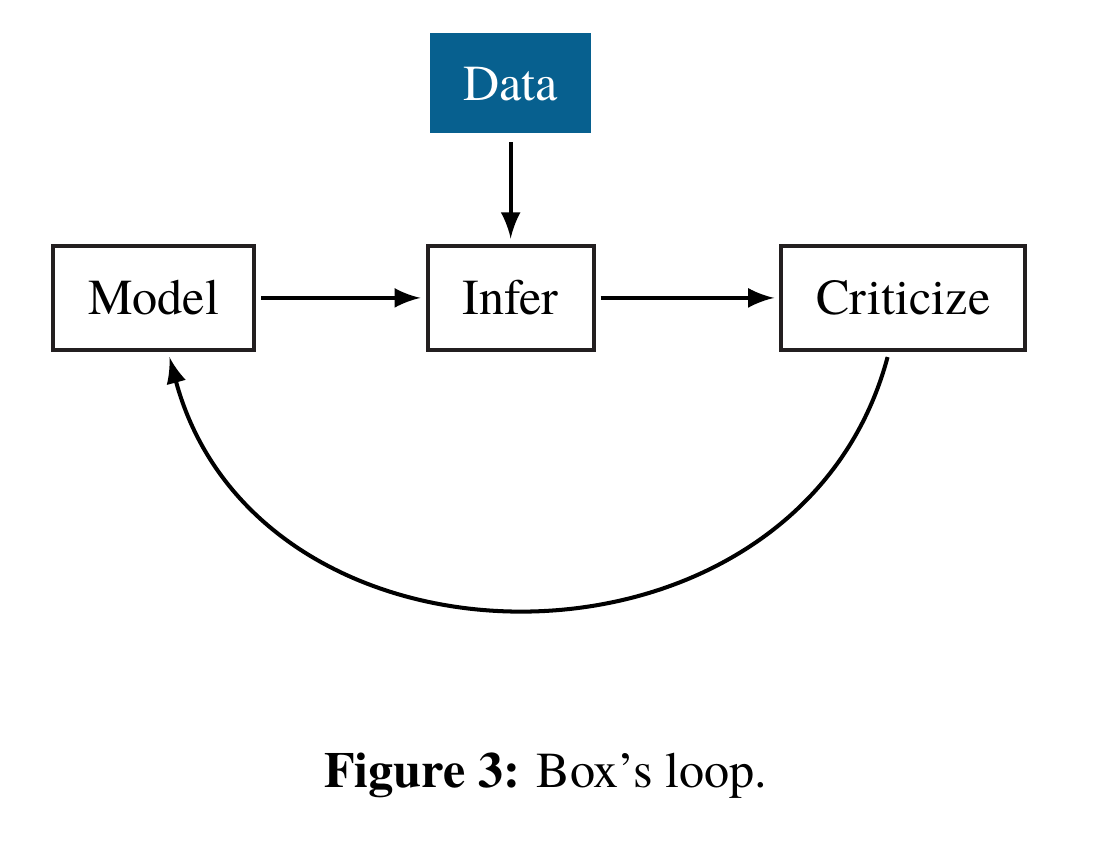
\includegraphics[scale=0.35]{boxs-loop.png}
\end{center}
\end{column}
\end{columns}
\tiny
\vspace{1cm}
\citep{Tran16,Blei14}
}

%%%%%%%%%%%%%%%%%%%%%%%%%%%%%%%%%%%%%%%%%%%%%%%%%%%%%%%%%%%%%%%%%%%%%%%%%%%%%%%
\frame{ 
\frametitle{Bayesian Inference}
\large \highlt{Degree of belief} \\ \ \\
\footnotesize
You are a skilled programmer, but bugs still slip into your code. After a particularly difficult implementation of an algorithm, you decide to test your code on a trivial example. It passes. You test the code on a harder problem. It passes once again. And it passes the next, \textit{even more difficult}, test too! You are \highlt{starting to believe} that there may be no bugs in this code...

\begin{flushleft}
\href{https://github.com/CamDavidsonPilon/Probabilistic-Programming-and-Bayesian-Methods-for-Hackers}{Bayesian methods for hackers}
\end{flushleft}

\begin{center}
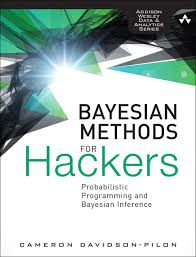
\includegraphics[scale=0.25]{bmh.jpeg}
\end{center}
}

%%%%%%%%%%%%%%%%%%%%%%%%%%%%%%%%%%%%%%%%%%%%%%%%%%%%%%%%%%%%%%%%%%%%%%%%%%%%%%%
\frame{ 
\frametitle{Some terminology}
\footnotesize

\begin{block}{Probabilistic model}
A joint distribution $p(X, \theta)$ of data $X$ and latent variables $\theta$.
\end{block}

\begin{equation}
P(\theta|x) = \frac{P(x|\theta)P(\theta)}{P(x)}
\end{equation}

\begin{itemize}
 \item \keywd{Prior} - $P(\theta)$ - one's beliefs about a quantity before presented with evidence
 \item \keywd{Posterior} - $P(\theta|x)$ - probability of the parameters given the evidence
 \item \keywd{Likelihood} - $P(x|\theta)$  - probability of the evidence given the parameters
 \item \keywd{Normalizing constant} - $P(x)$
\end{itemize}

\begin{itemize}
 \item $P(\theta)$: This big, complex code likely has a bug in it. 
 \item $P(\theta|X)$: The code passed all X tests; there still might be a bug, but it is less likely now.
\end{itemize}
}

%%%%%%%%%%%%%%%%%%%%%%%%%%%%%%%%%%%%%%%%%%%%%%%%%%%%%%%%%%%%%%%%%%%%%%%%%%%%%%%
\frame{
\frametitle{Related libraries and frameworks}
Libraries with high level of abstraction...
\begin{center}
Edward

\includegraphics[scale=0.1]{edward.png} \hspace{1cm}

\includegraphics[scale=0.3]{keras.png}
\end{center}
Computational framework libraries...
\begin{center}

\includegraphics[scale=0.3]{tensorflow.jpeg} \hspace{1cm}

\includegraphics[scale=0.3]{theano.jpeg} \hspace{1cm}

\includegraphics[scale=0.3]{torch.jpeg} 
\end{center}
}

%%%%%%%%%%%%%%%%%%%%%%%%%%%%%%%%%%%%%%%%%%%%%%%%%%%%%%%%%%%%%%%%%%%%%%%%%%%%%%%
\frame{
\frametitle{The three main probabilistic programming libraries}
\begin{center}
Edward

\includegraphics[scale=0.15]{edward.png} \hspace{1cm}

\includegraphics[scale=0.35]{stan.jpeg} \hspace{1cm} \\ \ \\

\includegraphics[scale=0.35]{pymc3.png}
\end{center}
}

%%%%%%%%%%%%%%%%%%%%%%%%%%%%%%%%%%%%%%%%%%%%%%%%%%%%%%%%%%%%%%%%%%%%%%%%%%%%%%%
\section{Model,Inference,Criticism}
\subsection{}

%%%%%%%%%%%%%%%%%%%%%%%%%%%%%%%%%%%%%%%%%%%%%%%%%%%%%%%%%%%%%%%%%%%%%%%%%%%%%%%
\begin{frame}[fragile]
\frametitle{PyMC3}
\footnotesize
\begin{code}
import pymc3 as pm
\end{code}

\begin{itemize}
 \item Developed by John Salvatier, Thomas Wiecki, and Christopher Fonnesbeck \citep{Salvatier16}
 \item Comes with \href{https://github.com/pymc-devs/pymc3/tree/master/pymc3/examples}{loads of good examples}
 \item API is is not backwards compartible with models specified in PyMC2
 \item Can still be run in Python2.7+.
\end{itemize}

\highlt{Basic workflow}
\begin{enumerate}
 \item Define hyperpriors
 \item Open a model context
 \item Perform inference
\end{enumerate}
\end{frame}

%%%%%%%%%%%%%%%%%%%%%%%%%%%%%%%%%%%%%%%%%%%%%%%%%%%%%%%%%%%%%%%%%%%%%%%%%%%%%%%
\begin{frame}[fragile]
\frametitle{Edward}
\footnotesize
\begin{block}{}
 Edward is named after the statistician \highlt{George Edward Pelham Box}. Its design is based on his philosophy of statistics
\end{block}
First gather data from some real-world phenomena. \ \\ 
Then cycle through \highlt{Box’s loop}
\begin{center}
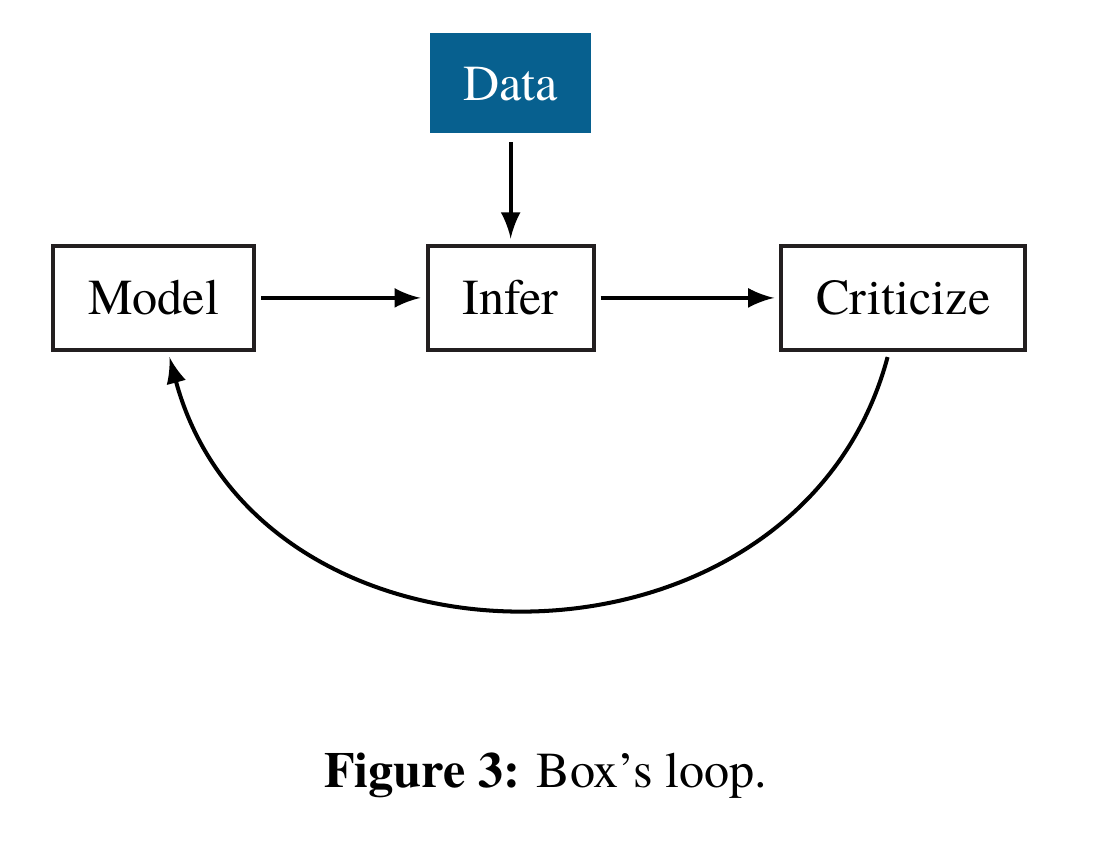
\includegraphics[scale=0.35]{boxs-loop.png}
\end{center}
\citep{Tran16}
\end{frame}

%%%%%%%%%%%%%%%%%%%%%%%%%%%%%%%%%%%%%%%%%%%%%%%%%%%%%%%%%%%%%%%%%%%%%%%%%%%%%%%
\begin{frame}[fragile]
\frametitle{Generalized procedure for probabilistic programming}
\footnotesize
\begin{block}{Model,Inference,Criticism}
\begin{enumerate}
 \item Build a probabilistic model of the phenomena
 \item Reason about the phenomena given model and data
 \item Criticize the model, revise and repeat
\end{enumerate}
\end{block}

A child flips a coin ten times...
\begin{code}
[0, 1, 0, 0, 0, 0, 0, 0, 0, 1]
\end{code}

\begin{enumerate}
 \item She is interested in the probability that the coin lands on heads
 \item Given she only see heads and tails she reason that a binomial distribution might be appropriate
 \item She finally analyzes whether her model captures the real-world phenomenon of coin flips (she may revise the model
and repeat)
\end{enumerate}
\citep{Tran16}
\end{frame}

%%%%%%%%%%%%%%%%%%%%%%%%%%%%%%%%%%%%%%%%%%%%%%%%%%%%%%%%%%%%%%%%%%%%%%%%%%%%%%%%
\frame{
\begin{center}
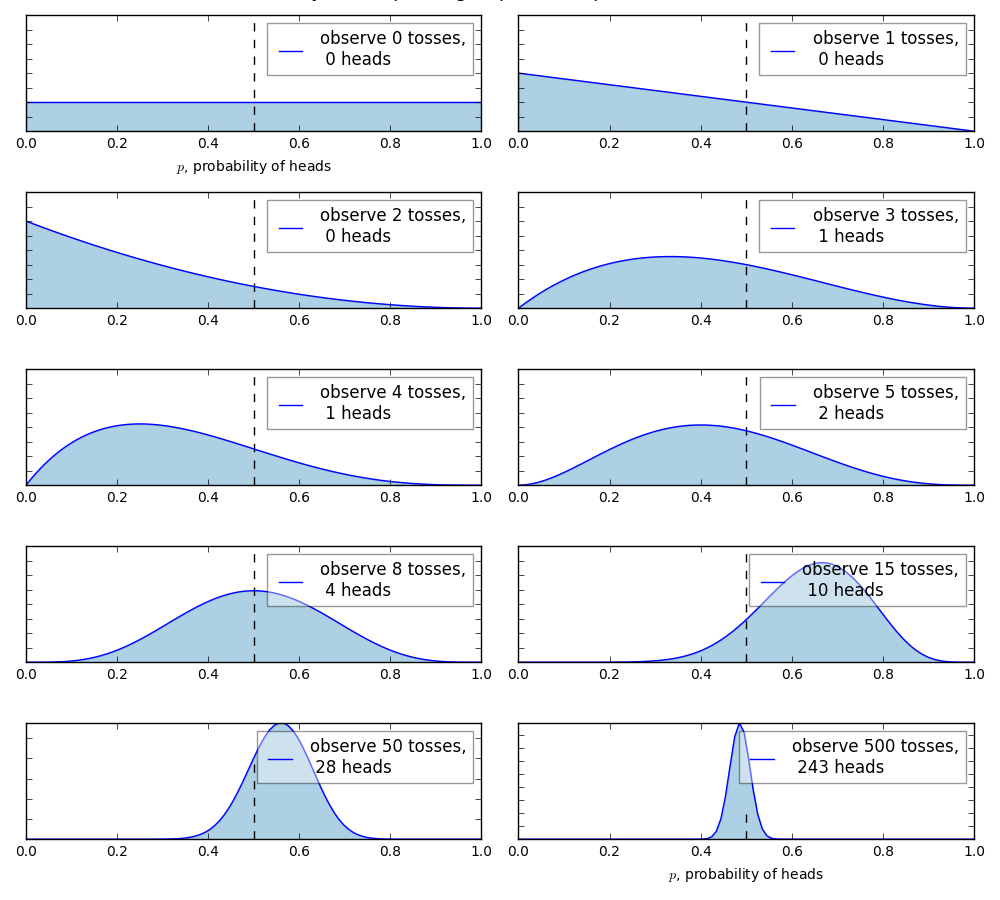
\includegraphics[scale=0.32]{coin_flip.png}
\end{center}
}

%%%%%%%%%%%%%%%%%%%%%%%%%%%%%%%%%%%%%%%%%%%%%%%%%%%%%%%%%%%%%%%%%%%%%%%%%%%%%%%
\begin{frame}[fragile]
\frametitle{Coin flip in PyMC3}
\footnotesize
\begin{code}
import pymc3 as pm

n,h,alpha,beta,niter = 100,61,2,2,1000

# context management
with pm.Model() as model: 
    p = pm.Beta('p', alpha=alpha, beta=beta)
    y = pm.Binomial('y', n=n, p=p, observed=h)

    start = pm.find_MAP()
    step = pm.Metropolis()
    trace = pm.sample(niter, step, start)
\end{code}

Data $\rightarrow$ Model context $\rightarrow$ Priors $\rightarrow$ Likelihood $\rightarrow$ Sampler $\rightarrow$ Inference
\vspace{0.5cm}
\\ \noindent To the notebooks!
\end{frame}

%%%%%%%%%%%%%%%%%%%%%%%%%%%%%%%%%%%%%%%%%%%%%%%%%%%%%%%%%%%%%%%%%%%%%%%%%%%%%%%
\begin{frame}[fragile]
\frametitle{Bayesian Linear Regression}
\scriptsize
For a set of $N$ data points $(\mathbf{X},\mathbf{y})=\{(\mathbf{x}_n, y_n)\}$, the model can be specified as follows: 

\begin{align}
 p(\mathbf{w})                         &= Normal(\mathbf{w}|\mathbf{0},\sigma_{w}^{2} \mathbf{I})\\
 p(b)                                  &= Normal(b|0,\sigma^{2}_{b}) \\
 p(\mathbf{y}|\mathbf{w},b,\mathbf{X}) &= \prod^{N}_{n=1} Normal(y_{n}|\mathbf{x}_{n}^{T} \mathbf{w} + b,\sigma^{2}_{y})
\end{align}

\begin{itemize}
 \item The latent variables are the linear model’s weights $\mathbf{w}$ and intercept $\mathbf{b}$
 \item We assume the prior and likelihood variances are known: $\sigma_{w}^{2}$, $\sigma_{b}^{2}$ and $\sigma^{2}_{y}$
 \item The mean of the likelihood is given by a linear transformation of the inputs in $\mathbf{x}_{n}$
\end{itemize}
\citep{Murphy12}
\end{frame}

% %%%%%%%%%%%%%%%%%%%%%%%%%%%%%%%%%%%%%%%%%%%%%%%%%%%%%%%%%%%%%%%%%%%%%%%%%%%%%%%%
% \frame{
% \frametitle{Bayes linear regression in Edward}
% \begin{center}
% 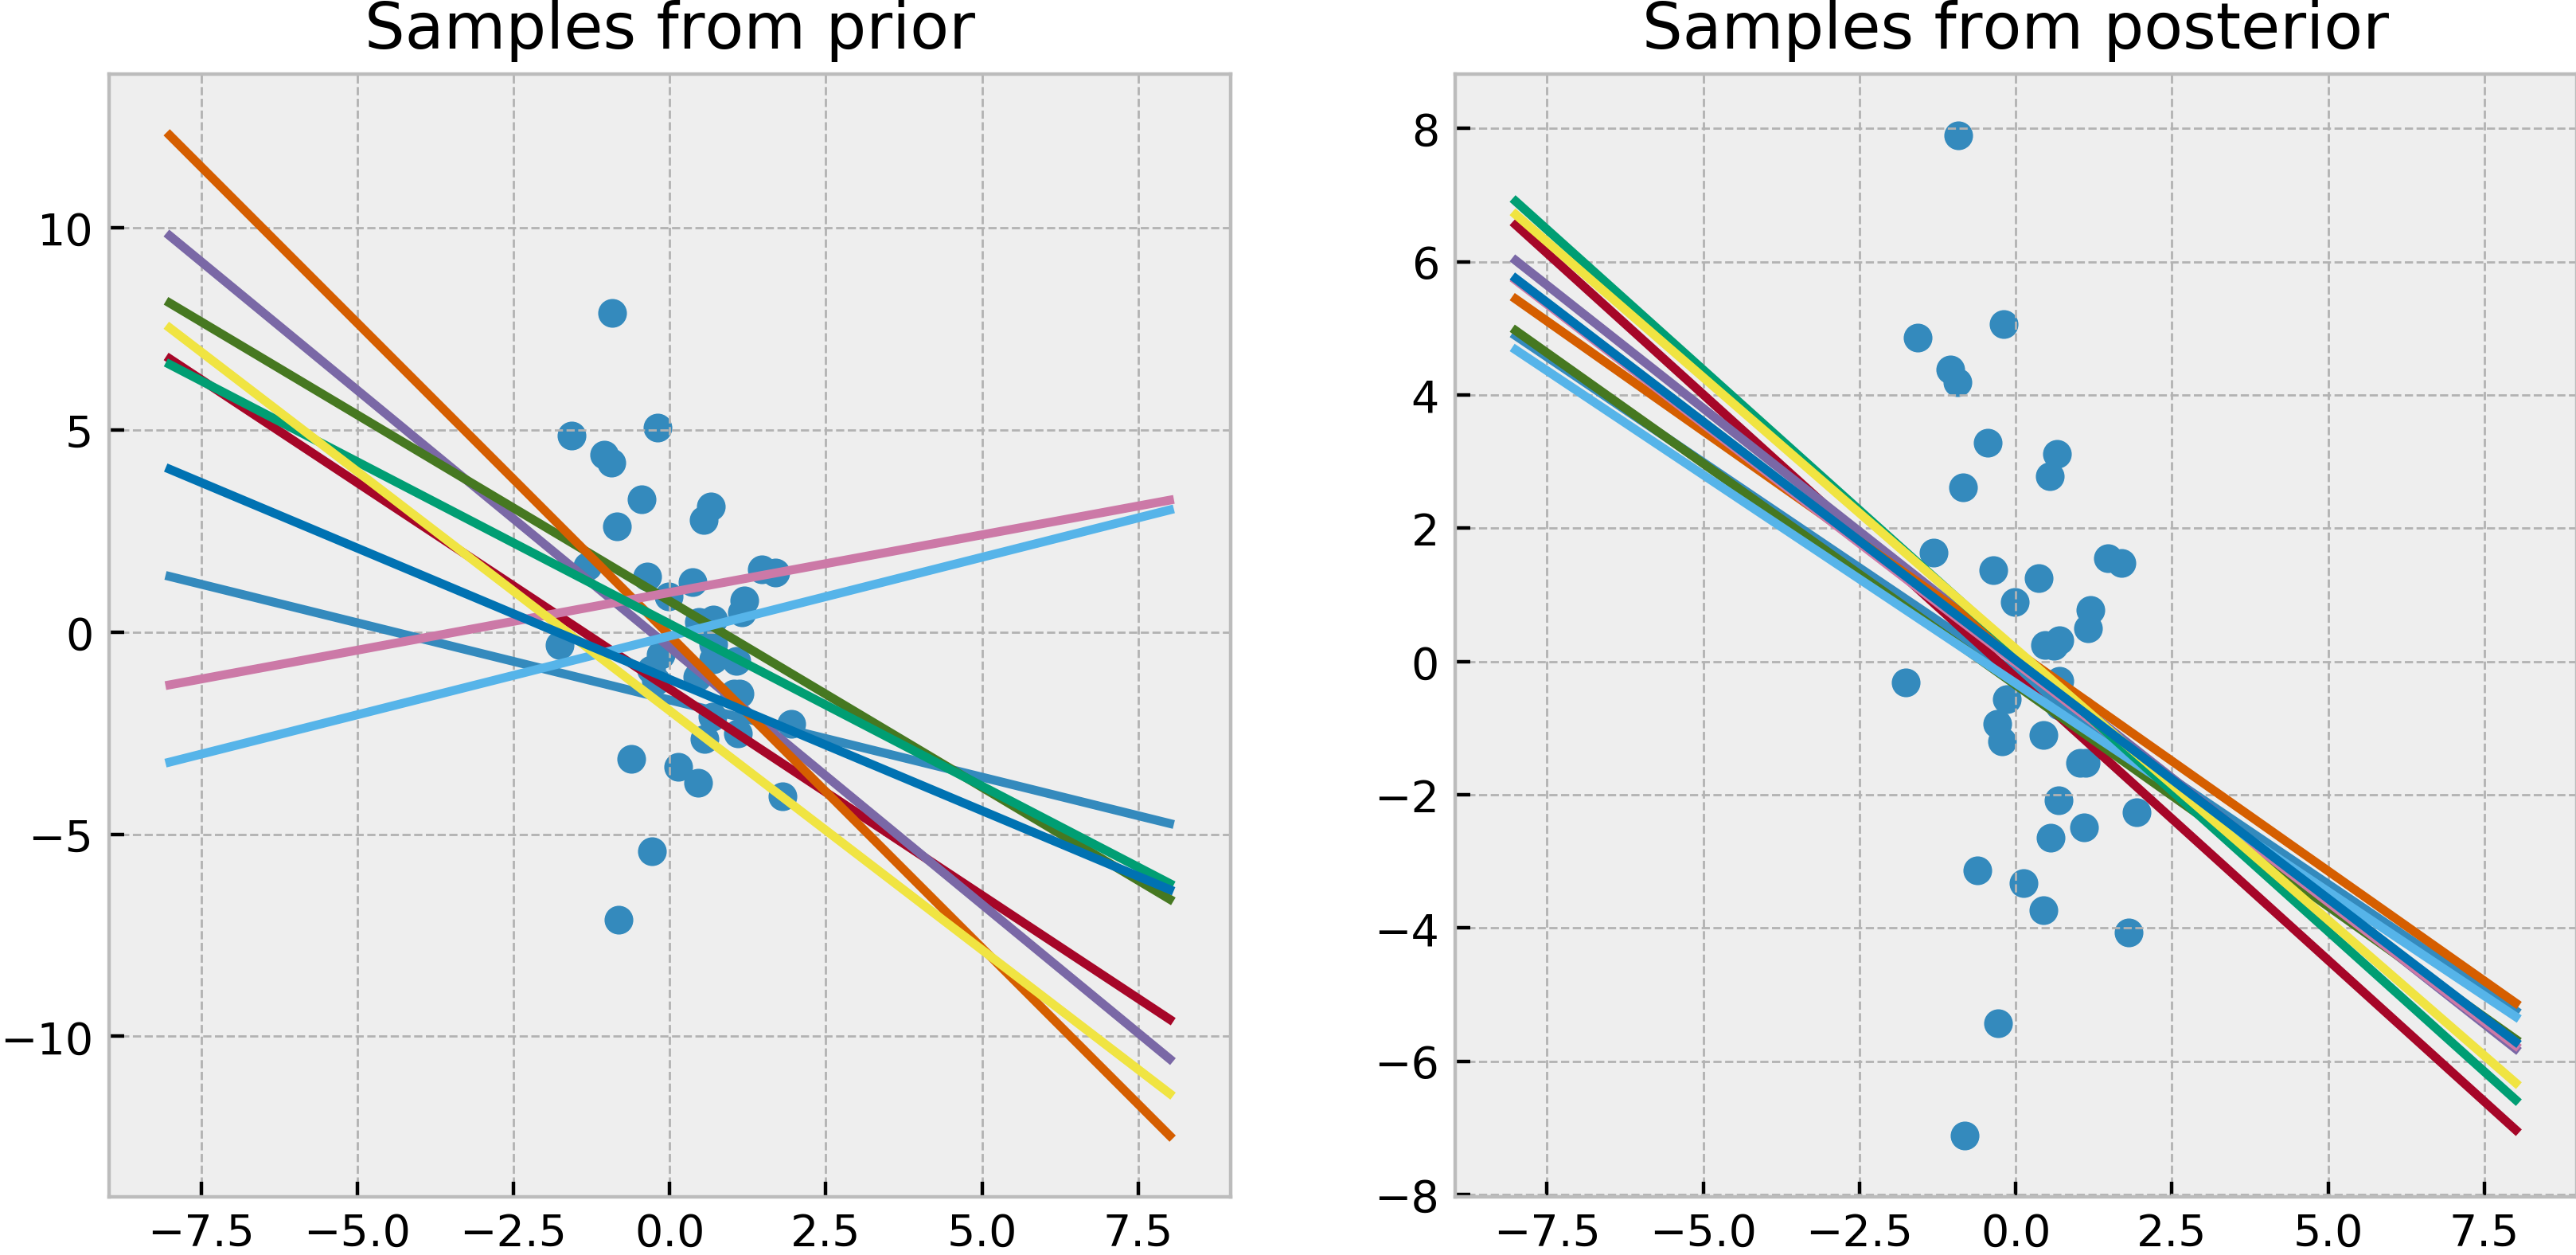
\includegraphics[scale=0.5]{../edward/bayes-linreg.png}
% \end{center}
% }

%%%%%%%%%%%%%%%%%%%%%%%%%%%%%%%%%%%%%%%%%%%%%%%%%%%%%%%%%%%%%%%%%%%%%%%%%%%%%%%%
\frame{
\frametitle{Bayes linear regression in PyMC3}
\begin{center}
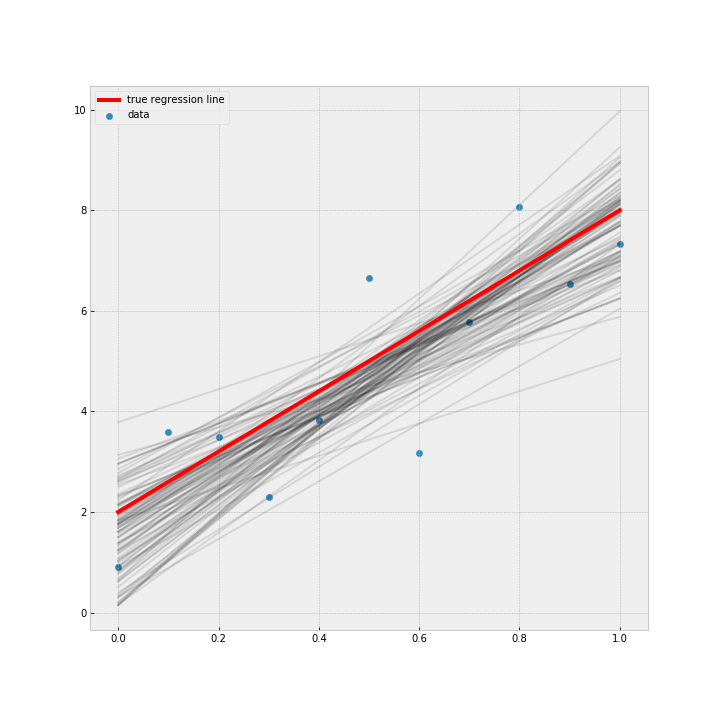
\includegraphics[scale=0.3]{../pymc3/bayes-lin-reg.png}
\end{center}
}

%%%%%%%%%%%%%%%%%%%%%%%%%%%%%%%%%%%%%%%%%%%%%%%%%%%%%%%%%%%%%%%%%%%%%%%%%%%%%%%
\frame{
\frametitle{Markov chain Monte Carlo (MCMC)}
\footnotesize
\keywd{MCMC}
\begin{itemize}
 \item It is a family of algorithms for obtaining a sequence of random samples from a probability distribution for which direct sampling is difficult.
 \item The sequence can then be used to approximate the distribution
 \item It allows for inference on complex models
\end{itemize}

A particularly useful class of MCMC, known as Hamliltonian Monte Carlo, requires \href{https://en.wikipedia.org/wiki/Gradient}{gradient} information which is often not readily available so PyMC3 uses Theano to get around this problem.  Something that has recently made this whole field a lot more interesting is the No-U-turn sampler (NUTS) because there are \highlt{self-tuning strategies} \citep{Hoffman14}.
\\ \ \\
One of the really nice things about probabilistic programming is that \highlt{you do not have to know how inference is performed}, but it can be useful.  

\begin{itemize}
 \item \href{http://twiecki.github.io/blog/2015/11/10/mcmc-sampling/}{MCMC for Dummies}
 \item \href{https://arxiv.org/pdf/1206.1901.pdf}{More on Hamliltonian MCMC (Not for dummies)}
 \item \href{http://twiecki.github.io/blog/2014/01/02/visualizing-mcmc/}{How to animate MCMC (for everyone)}
\end{itemize}
}

%%%%%%%%%%%%%%%%%%%%%%%%%%%%%%%%%%%%%%%%%%%%%%%%%%%%%%%%%%%%%%%%%%%%%%%%%%%%%%%%
\frame{
\frametitle{There are a lot of tools for inference available}
\footnotesize
\begin{center}
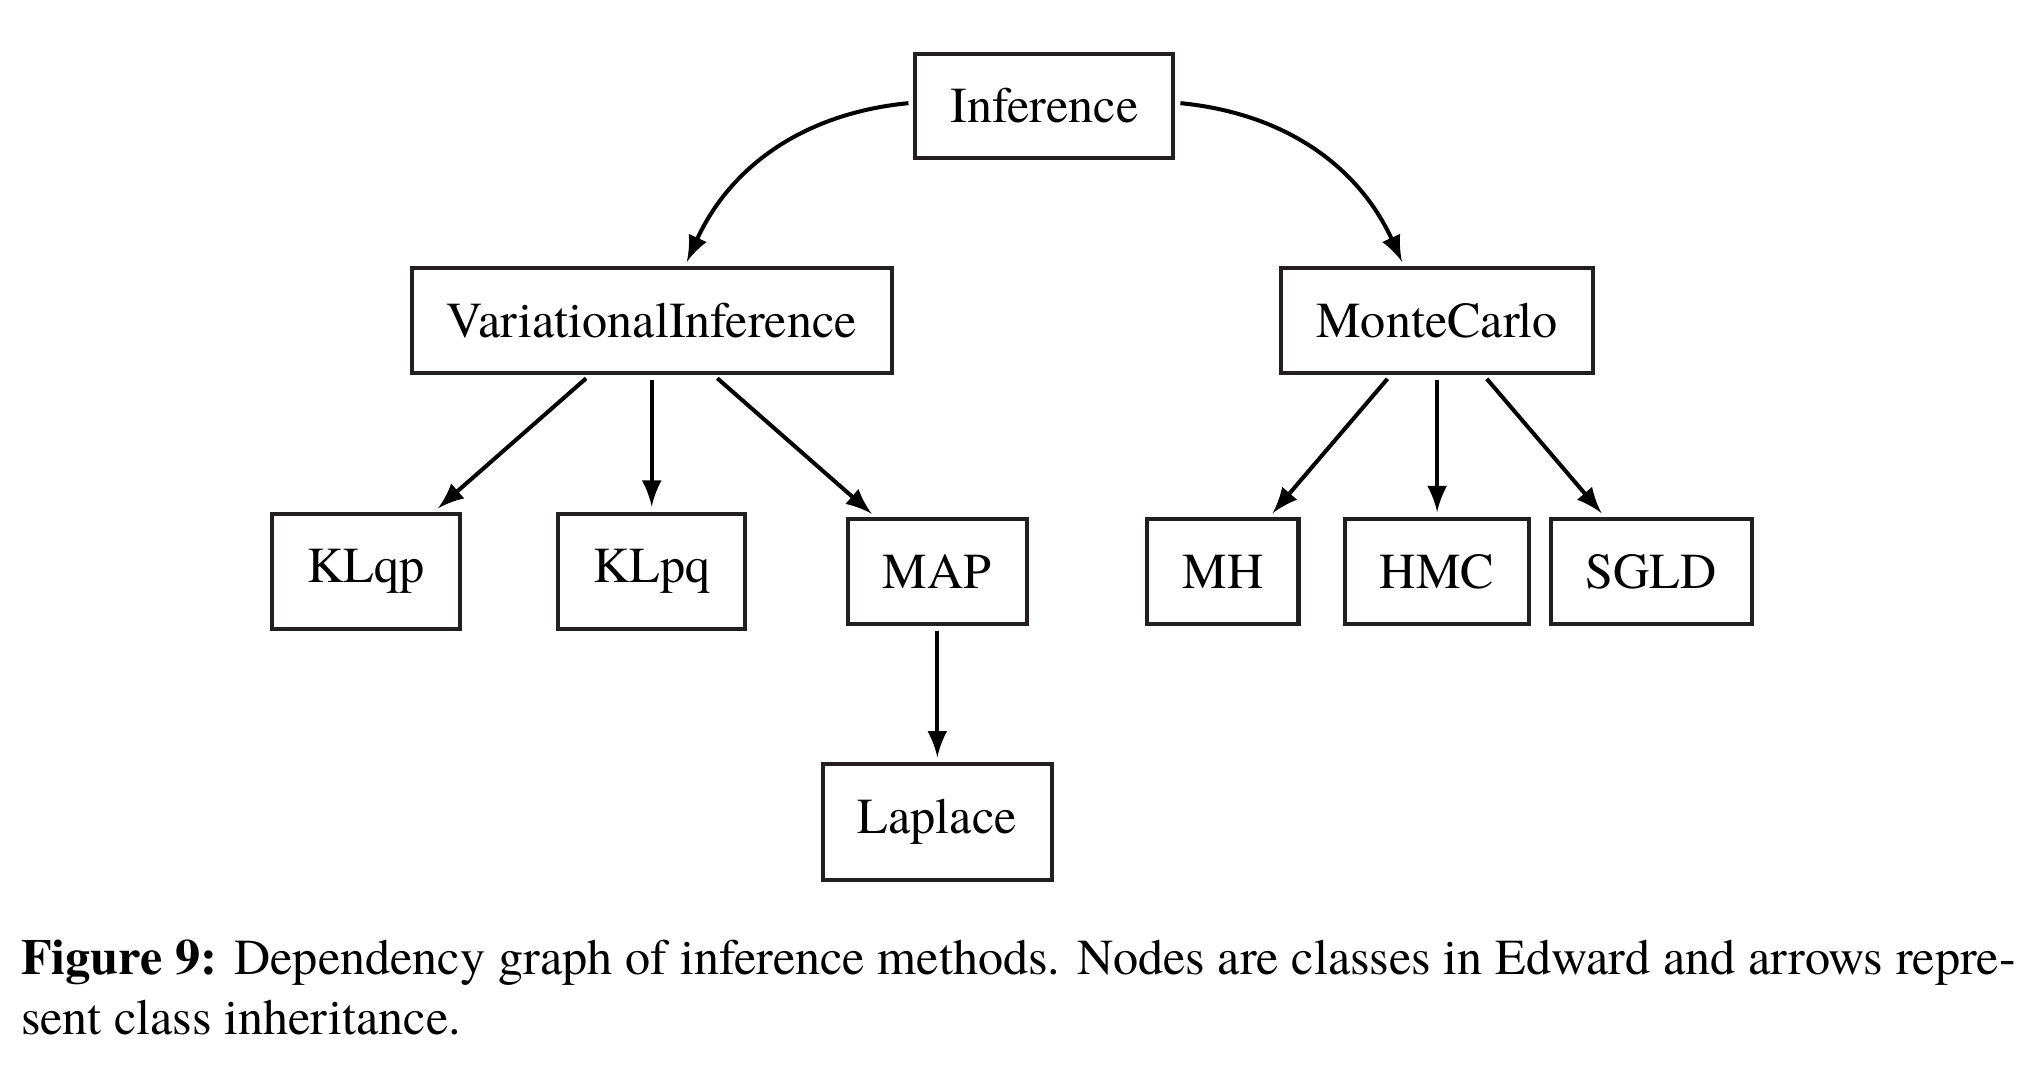
\includegraphics[scale=0.4]{inference-graph.png}
\end{center}
%\vspace{1cm}
\citep{Tran16}
}

%%%%%%%%%%%%%%%%%%%%%%%%%%%%%%%%%%%%%%%%%%%%%%%%%%%%%%%%%%%%%%%%%%%%%%%%%%%%%%%
\begin{frame}[fragile]
 \footnotesize
 
 \begin{block}{Bayes Factor}
  It is the \keywd{Bayesian way} to compare models.   This is done by computing the marginal likelihood of each model 
  \begin{equation}
  BF = \frac{p(y|M_{0})}{p(y|M_{1})}
  \end{equation}
  \highlt{Can be used to replace the p-value}
 \end{block}

 \begin{block}{Posterior predictive checks}
  Analyze the degree to which data generated from the model deviate from data generated from the true distribution. Can by used for hypothesis testing, model comparison, model selection, model averaging and to validate test data.
 \end{block}

Links
\begin{itemize}
 \item \href{http://docs.pymc.io/notebooks/Bayes\_factor.html}{Bayes Factor in PyMC3}
 \item \href{http://docs.pymc.io/notebooks/posterior\_predictive.html}{Posterior predictive checks in PyMC3}
 \item \href{https://replicationindex.wordpress.com/2015/04/30/replacing-p-values-with-bayes-factors-a-miracle-cure-for-the-replicability-crisis-in-psychological-science/}{replacing p-values}
 \item \href{http://docs.pymc.io/notebooks/BEST.html}{Bayesian estimation supersedes the t-test}
\end{itemize}
\end{frame}

%%%%%%%%%%%%%%%%%%%%%%%%%%%%%%%%%%%%%%%%%%%%%%%%%%%%%%%%%%%%%%%%%%%%%%%%%%%%%%%
\section{Decisions, Decisions}
\subsection{}

%%%%%%%%%%%%%%%%%%%%%%%%%%%%%%%%%%%%%%%%%%%%%%%%%%%%%%%%%%%%%%%%%%%%%%%%%%%%%%%
\begin{frame}[fragile]
\footnotesize
\begin{block}{}
We can never validate whether a model is true.
\\ \ \\
\keywd{In practice, all models are wrong -George Box}.
\\ \ \\
However, we can try to uncover where the model goes wrong. Model criticism helps justify the
model as an approximation or point to good directions for revising the model.
\end{block}
\vspace{1cm}
Posterior predictive checks (PPCs) analyze the degree to which data generated from the model deviate
from data generated from the true distribution. They can be used either numerically to quantify this
degree, or graphically to visualize this degree.
\end{frame}

%%%%%%%%%%%%%%%%%%%%%%%%%%%%%%%%%%%%%%%%%%%%%%%%%%%%%%%%%%%%%%%%%%%%%%%%%%%%%%%
\begin{frame}[fragile]
\footnotesize
\frametitle{RMSE and MSE}
Model evaluation has become so much easier...
\vspace{1cm}
\begin{code}
print("Mean squared error on test data:")
print(ed.evaluate('MSE', data={X: X_test, y_post: y_test}))
\end{code}

\begin{code}
print("Mean absolute error on test data:")
print(ed.evaluate('MAE', data={X: X_test, y_post: y_test}))
\end{code}
\vspace{1cm}
Note: RMSE gives a relatively high weight to large errors. This means the RMSE should be more useful when large errors are particularly undesirable.
\end{frame}

%%%%%%%%%%%%%%%%%%%%%%%%%%%%%%%%%%%%%%%%%%%%%%%%%%%%%%%%%%%%%%%%%%%%%%%%%%%%%%%
\begin{frame}[fragile]
\begin{block}{Switchpoint analysis}
\footnotesize
\begin{itemize}
 \item \href{http://nbviewer.jupyter.org/github/CamDavidsonPilon/Probabilistic-Programming-and-Bayesian-Methods-for-Hackers/blob/master/Chapter1\_Introduction/Ch1\_Introduction\_PyMC3.ipynb}{Probabilistic Programming and Bayesian Methods for Hackers \\ Text Messages}
 \item \href{http://docs.pymc.io/notebooks/getting_started.html}{PyMC3 Documentation \\ Coal Mining Disasters}
\end{itemize}
\end{block}
\end{frame}

%%%%%%%%%%%%%%%%%%%%%%%%%%%%%%%%%%%%%%%%%%%%%%%%%%%%%%%%%%%%%%%%%%%%%%%%%%%%%%%
\begin{frame}[fragile]
\frametitle{Switchpoint analysis applications}
\begin{block}{}
\begin{itemize}
 \item Did the change actually happen?
 \item Did change X on January 1 affect the number of sales we have seen in our company?
 \item Did imposing a new safety policy last summer reduce the number of accidents?
 \item After those staffing decisions how longs did it take before revenue was affected?
 \item Based on my time-series forecasting model when will a change actually occur?
 \item ...
\end{itemize}
\end{block}
\begin{block}{}
If $p$-values are your tool of choice you could try Bayes Factors to have numeric values to make decisions from.
\end{block}
\end{frame}

%%%%%%%%%%%%%%%%%%%%%%%%%%%%%%%%%%%%%%%%%%%%%%%%%%%%%%%%%%%%%%%%%%%%%%%%%%%%%%%
\begin{frame}[fragile]
\begin{block}{Multilevel modeling}
Multilevel model. Multilevel models (also known as hierarchical linear models, nested data models, mixed models, random coefficient, random-effects models, random parameter models, or split-plot designs) are statistical models of parameters that vary at more than one level
\end{block}
\vspace{1cm}
\begin{itemize}
 \item \href{http://twiecki.github.io/blog/2014/03/17/bayesian-glms-3/}{PyMC3 - Radon example GLM style}
 \item \href{http://edwardlib.org/tutorials/linear-mixed-effects-models}{Edward - Instructor evaluation ratings}
\end{itemize}
\vspace{1cm}
\href{https://en.wikipedia.org/wiki/Multilevel\_model}{https://en.wikipedia.org/wiki/Multilevel\_model}
\end{frame}

%%%%%%%%%%%%%%%%%%%%%%%%%%%%%%%%%%%%%%%%%%%%%%%%%%%%%%%%%%%%%%%%%%%%%%%%%%%%%%%
\begin{frame}[fragile]
\frametitle{A note on deep learning...}
\begin{enumerate}
 \item Neural Networks compute point estimates
 \item They tend to be overly confident about class prediction
 \item They are prone to overfitting
 \item They have many parameters that may require tuning
\end{enumerate}

\begin{block}{}
 How confident am I in my prediction---can I quantify the uncertainty?
\end{block}

\keywd{Bayesian neural network}: Is a neural network with a prior distribution on the weights

\tiny
\href{https://www.youtube.com/watch?v=I09QVNrUS3Q}{https://www.youtube.com/watch?v=I09QVNrUS3Q}
\citep{Tran17}
\end{frame}

%%%%%%%%%%%%%%%%%%%%%%%%%%%%%%%%%%%%%%%%%%%%%%%%%%%%%%%%%%%%%%%%%%%%%%%%%%%%%%%%
\frame{
\frametitle{Simple Neural Network using PyMC3}
\footnotesize
\begin{center}
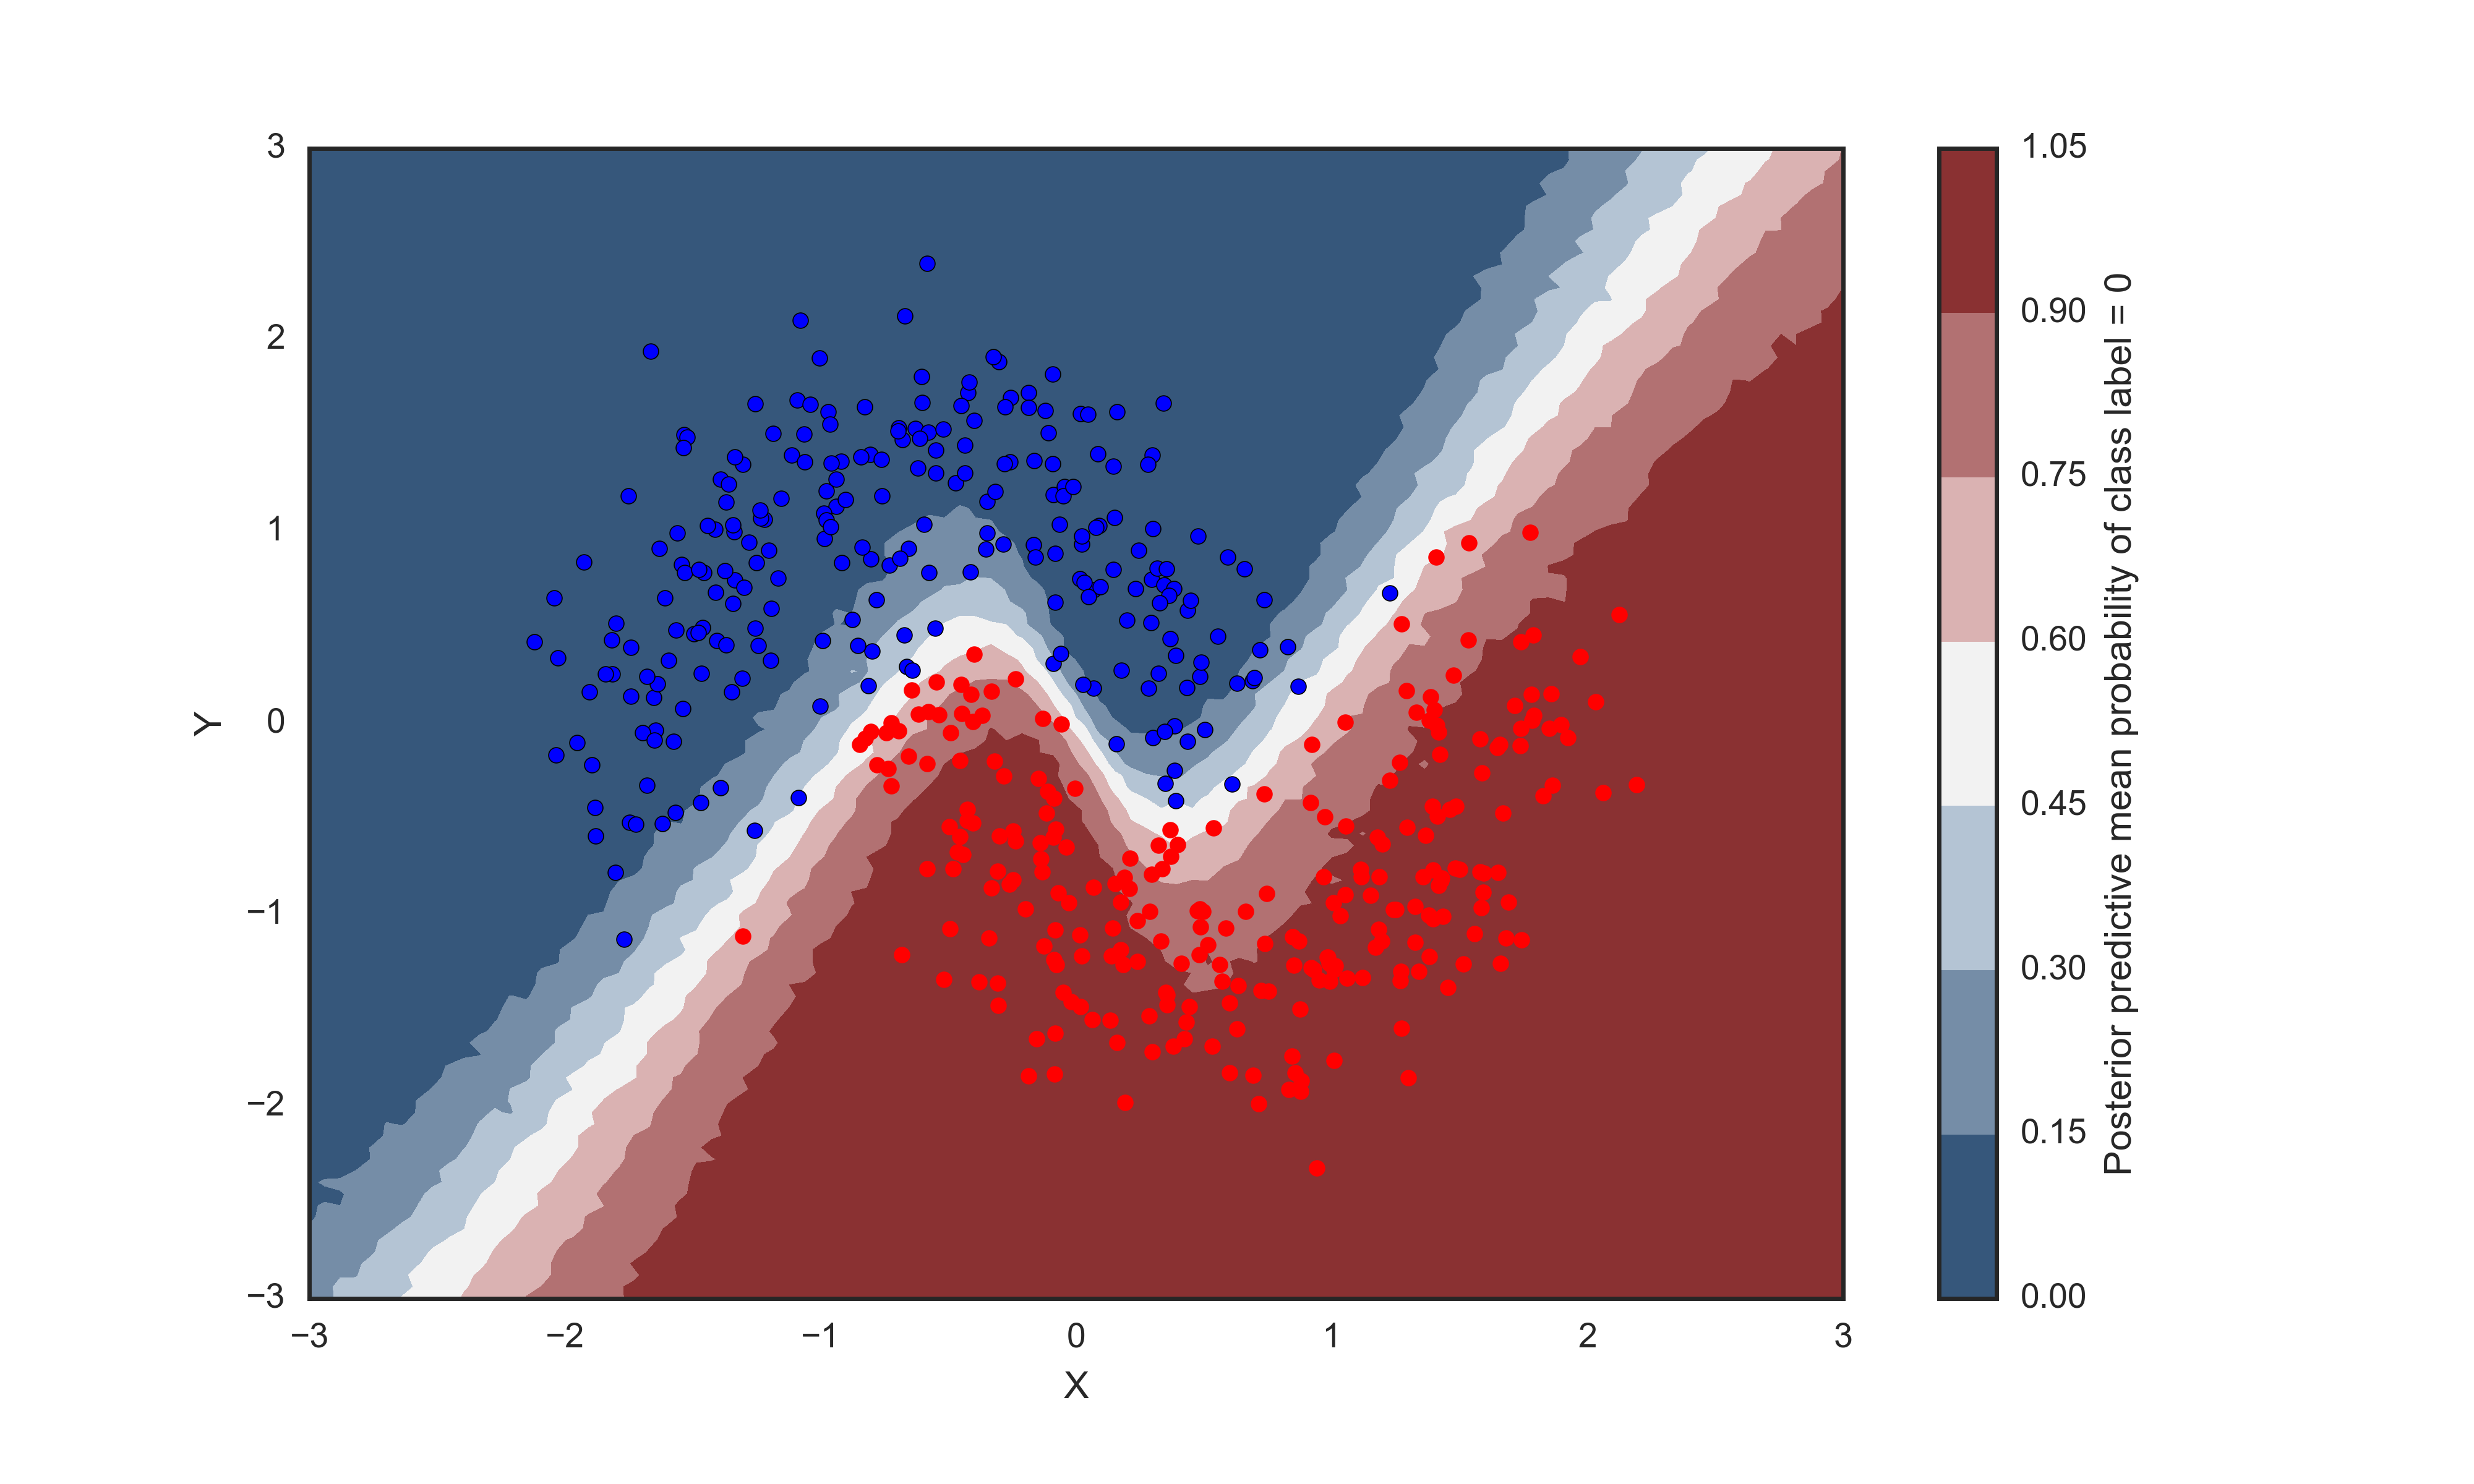
\includegraphics[scale=0.2]{../pymc3/nn-1.png}
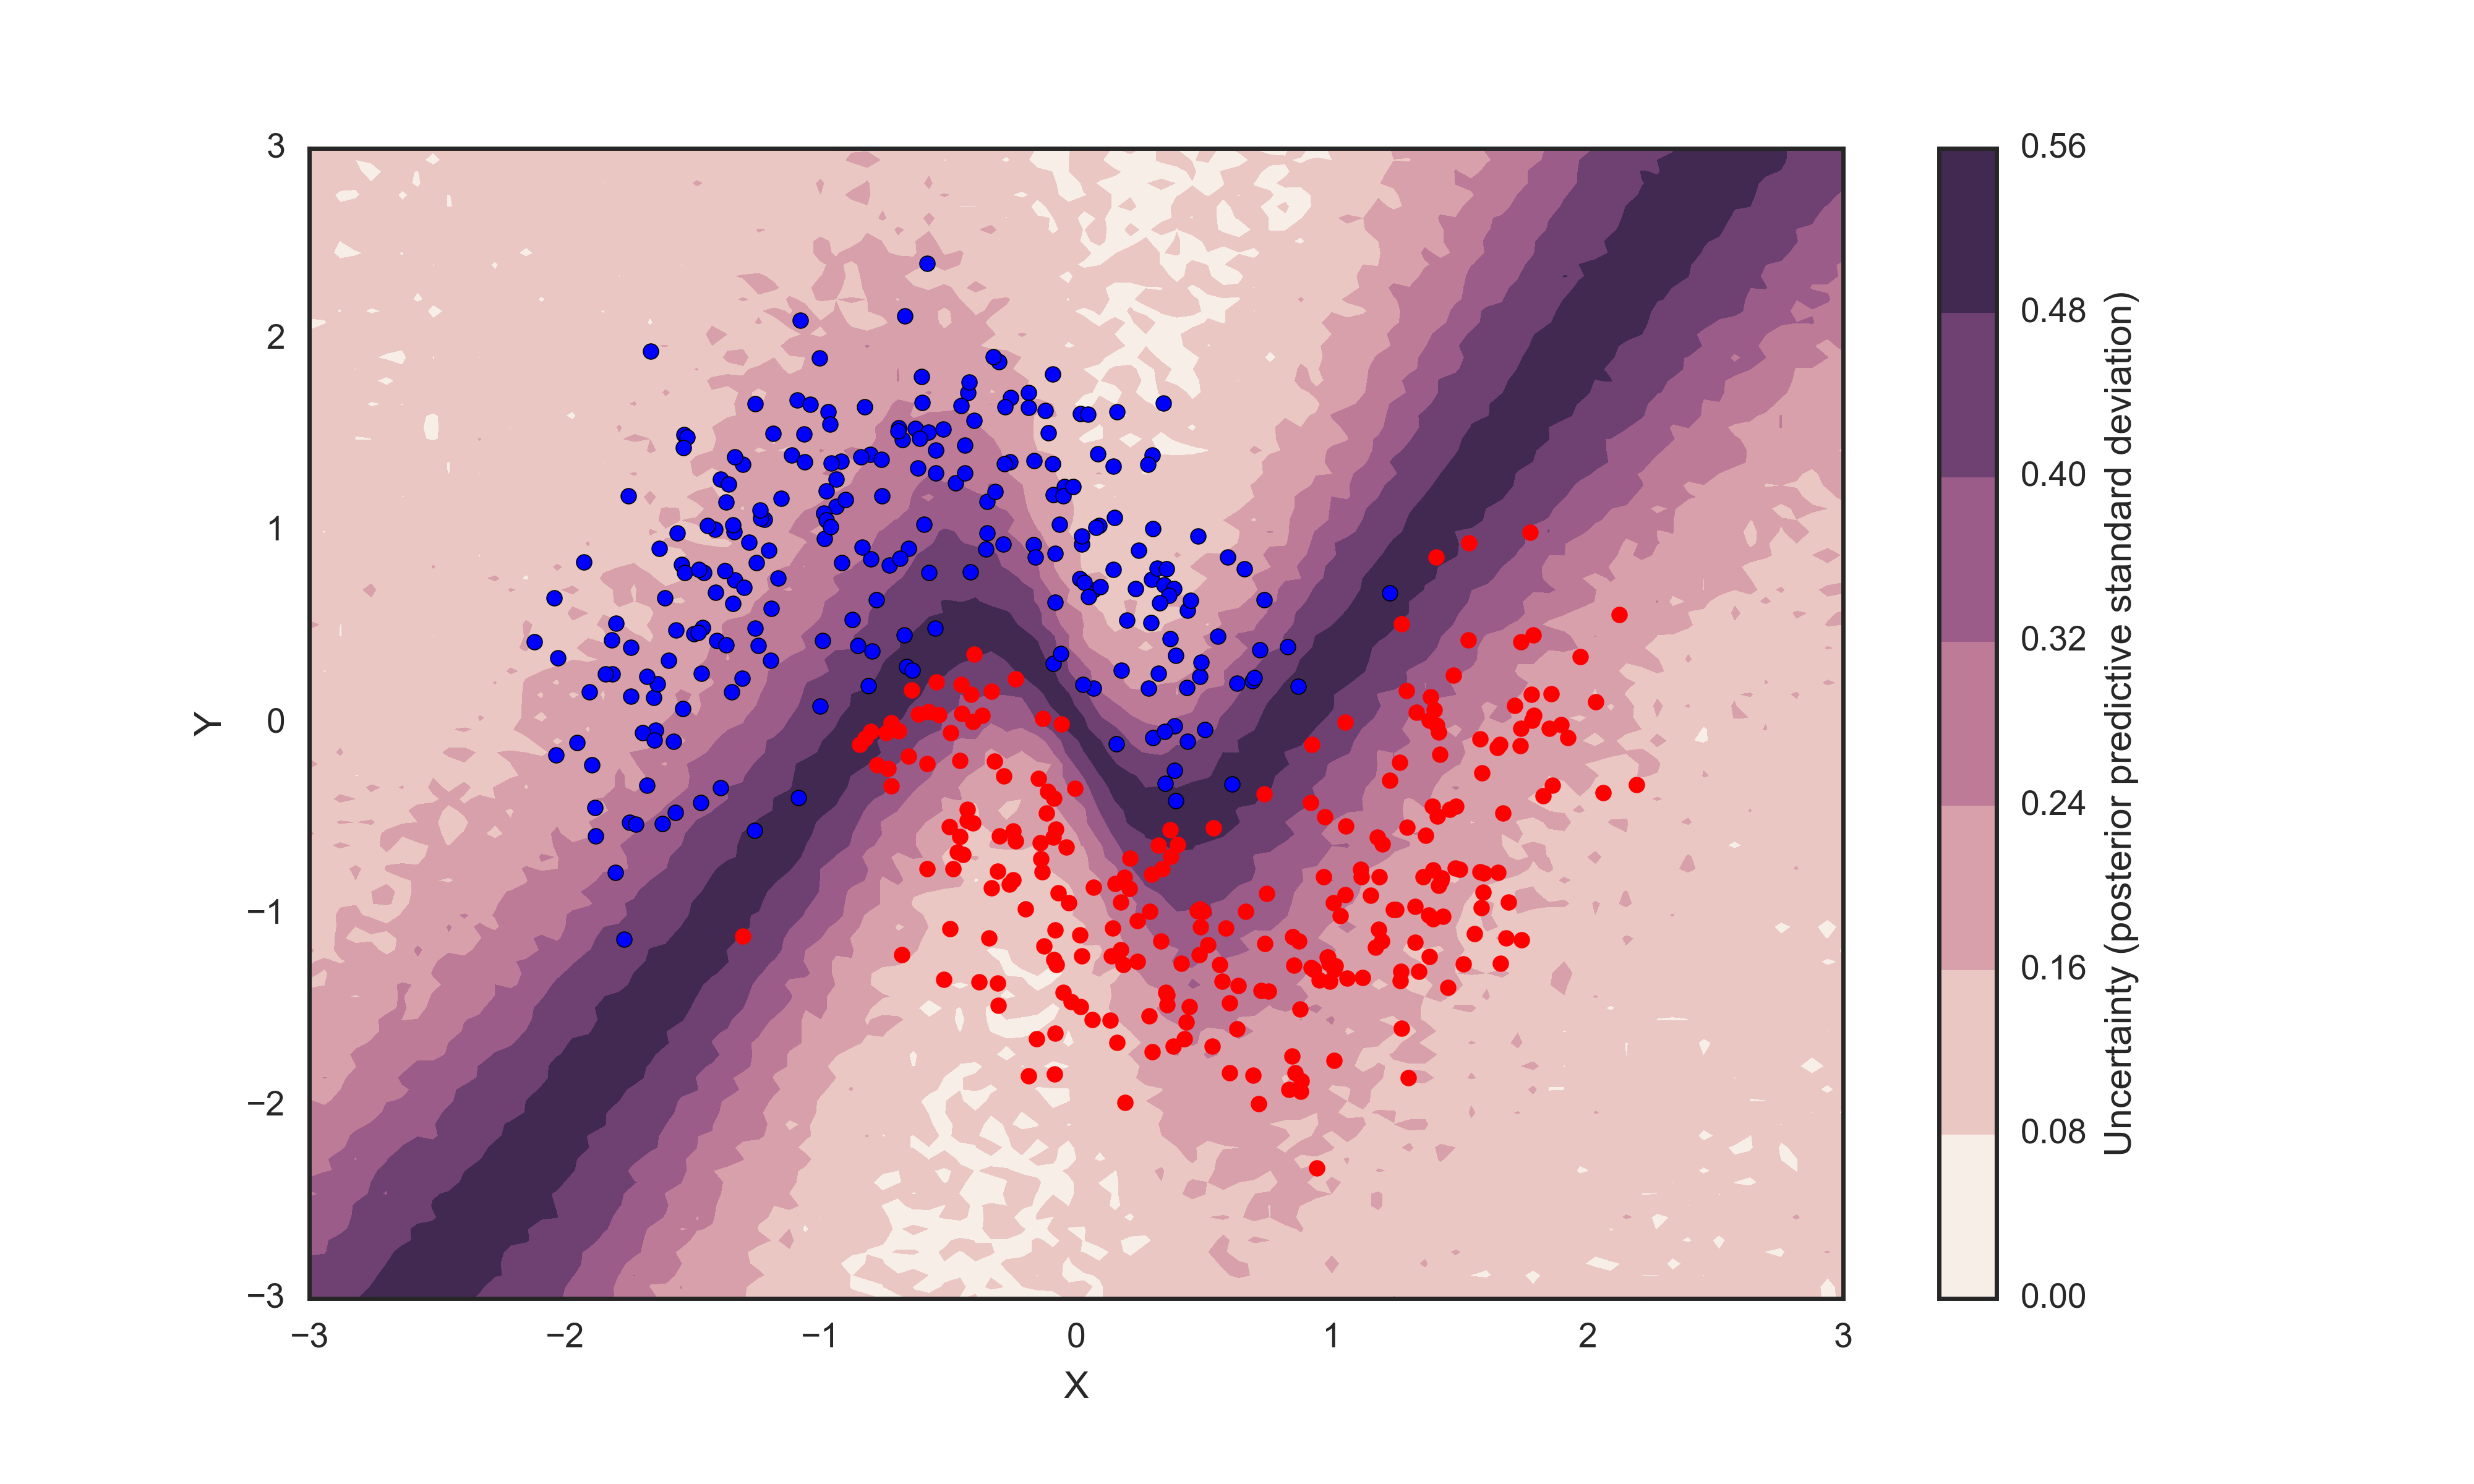
\includegraphics[scale=0.2]{../pymc3/nn-2.png}
\end{center}
}

%%%%%%%%%%%%%%%%%%%%%%%%%%%%%%%%%%%%%%%%%%%%%%%%%%%%%%%%%%%%%%%%%%%%%%%%%%%%%%%
\frame{ 
\frametitle{Another take on probabilistic programming}
\footnotesize
\begin{block}{}
 Another way of thinking about this: unlike a traditional program, which only runs in the forward directions, \highlt{a probabilistic program is run in both the forward and backward direction}. It runs forward to compute the consequences of the assumptions it contains about the world (i.e., the model space it represents), but it also runs backward from the data to constrain the possible explanations. In practice, many probabilistic programming systems will cleverly interleave these forward and backward operations to efficiently home in on the best explanations.
\end{block}
\vspace{1cm}
\href{https://plus.google.com/u/0/107971134877020469960/posts/KpeRdJKR6Z1}{Why Probabilistic Programming matters? (Beau Cronin)}
}

%%%%%%%%%%%%%%%%%%%%%%%%%%%%%%%%%%%%%%%%%%%%%%%%%%%%%%%%%%%%%%%%%%%%%%%%%%%%%%%
\frame{   
\frametitle{What did we cover again?}
\begin{block}{}
 \begin{itemize}
  \item[\checkmark] Probabilistic programming intro
  \item[\checkmark] Box's Loop (Model $\rightarrow$ infer $\rightarrow$ criticize)
  \item[\checkmark] Bayesian inference and some related tools
  \item[\checkmark] Examples in both PyMC3 and Edward (model)
  \item[\checkmark] Discuss the tools used for inference and criticism
  \item[\checkmark] Switchpoint and multilevel modeling examples
  \end{itemize}
\end{block}
}

%%%%%%%%%%%%%%%%%%%%%%%%%%%%%%%%%%%%%%%%%%%%%%%%%%%%%%%%%%%%%%%%%%%%%%%%%%%%%%%
\frame{ 
\frametitle{Where to go from here}
\footnotesize

Examples, examples, examples...
\begin{itemize}
 \item \href{http://edwardlib.org/tutorials/}{Edward examples}
 \item \href{https://github.com/pymc-devs/pymc3}{PyMC3 examples}
 \item \href{http://pymc-devs.github.io/pymc3/notebooks/getting_started.html}{PyMC3 Getting started guide}
 \item \href{https://github.com/CamDavidsonPilon/Probabilistic-Programming-and-Bayesian-Methods-for-Hackers}{Bayesian methods 
for hackers}
  \item \href{http://twiecki.github.io}{Blog by Thomas Wiecki}
  \item \href{http://www.amazon.com/Doing-Bayesian-Analysis-Second-Edition/dp/0124058884/ref=dp_ob_title_bk}{Doing Bayesian Data Analysis by John Kruschke}
  \item \href{https://github.com/markdregan/Bayesian-Modelling-in-Python}{Resource by Mark Dregan}
  \item This is \href{http://www.kdnuggets.com/2016/12/datascience-introduction-bayesian-inference.html}{a nice intro to Bayesian thinking done on kdnuggets (using PyMC3)}
\end{itemize}

There is also \href{https://github.com/stan-dev/example-models/wiki}{PyStan} (\href{http://www.stat.columbia.edu/~gelman/research/unpublished/stan-resubmit-JSS1293.pdf}{Stan paper})
}

%%%%%%%%%%%%%%%%%%%%%%%%%%%%%%%%%%%%%%%%%%%%%%%%%%%%%%%%%%%%%%%%%%%%%%%%%%%%%%%%
\frame{
\frametitle{Galvanize}
\footnotesize
\begin{block}{Upcoming events}
 \begin{itemize}
  \item \keywd{Essential Mathematical Foundations for Data Science} (January 08-10)
  \item \keywd{Intro to Tableau for Data Science} (January 11th)
  \item \keywd{Statistics short-course} (January 22-24)
  \item \keywd{Intro to Python - Part time Course} (February-March)
  \item \keywd{Data Science Immersive} (February-May)
 \end{itemize}
\end{block}
}

%%%%%%%%%%%%%%%%%%%%%%%%%%%%%%%%%%%%%%%%%%%%%%%%%%%%%%%%%%%%%%%%%%%%%%%%%%%%%%
\frame[allowframebreaks]{
\frametitle{References}
\begin{tiny} \bibliography{pp.bib}
\bibliographystyle{apalike}         % Style BST file
\end{tiny}
}

\end{document}